\silentchapter{6 Forma oppstår mellom agentane}{forma oppstår mellom agentane}

\prop{6}{}{Forma oppstår i feltet mellom agentar.}

Ingen stol er laga av éin agent. Bøketreet dreg i éin retning; det tillèt bøyingar langs fiberen men vetoar brot på tvers. Dampkjelen dreg i ei anna; han opnar moglege buktingar som treet åleine forbyr. Stolmakaren dreg i ei tredje; han navigerer mot ein konfigurasjon som forløyser alle trykka han kan sjå. Kunden dreg i ei fjerde; ho vel blant dei formene marknaden tilbyr. Ingen av dei dikterer utfallet. Forma er det som trer fram i skjeringspunktet mellom alle desse kreftene samstundes.

Denne innsikta; at forma ikkje er designa av nokon, men oppstår mellom agentar; er det som skil dette rammeverket frå tradisjonell designteori. Tradisjonell teori spør kva designaren ville. Me spør kva feltet produserte. Designaren er éin agent blant mange; ein viktig agent, men aldri den einaste.

\section*{Det poly-agentiske kompromisset}

\prop{6.1}{t}{Fleire agentar responderer på ulike trykk samstundes. Kvar form er eit poly-agentisk kompromiss. Ingen einskild agent dikterer morfologien; ho trer fram i skjeringspunktet mellom dei.}

La oss gå attende til Thonet nr. 14. Dei identifiserbare agentane inkluderer: bøketreet (vetoar og tillèt via fiberstruktur); dampen (temporært endrar materialaffordansen); dreiemaskinen (standardiserer komponentdiameter); Thonet sjølv (navigerer med ein lyskjegle over kostnad, montering, transport og visuell karakter); fabrikkarbeidaren (utfører regelapplikasjonar i produksjonskjeda); kaféverten (selekterer for stablingsevne og visuell lettheit); transportøraren (selekterer for flatpakking og volum); og sluttbrukaren (selekterer for sitjekomfort og sosial signalisering).

Kvar av desse agentane opererer innanfor si eiga lyskjegle. Bøketreet «ser» berre fiberretning og fukt. Dampen «ser» berre temperatur og trykk. Thonet ser kostnad, montering, transport og form. Kaféverten ser stabling og sosial kontekst. Ingen av dei har ein global representasjon av det endelege produktet. Likevel konvergerer dei mot ein stabil posisjon i formrommet som har vart i over 160 år.

\prop{6.11}{t}{Kvart nivå løyser problem kompetent innanfor si eiga lyskjegle. Lågare komponentar fremjar mål dei manglar kapasitet til å representere. Reduksjonisme og holisme er komplementære; begge er sanne, ingen er tilstrekkeleg åleine.}

Korleis er dette mogleg? Korleis kan agentar utan global oversikt produsere ein globalt stabil form? Svaret er at kvart nivå løyser problem kompetent innanfor sitt eige domene. Bøketreet «veit ikkje» at det bidreg til ein stol. Det responderer utelukkande på fukt, temperatur og mekanisk stress. Men responsen er kompetent: den produserer kurver som i neste ledd gjev stolen sine karakteristiske bøyingar. Treet fremjar eit mål det manglar kapasitet til å representere.

Dette er kjernen i Michael Levins multiskala-kompetansearkitektur. Kvart nivå i eit biologisk system; frå celler via vev til organ til organismar; er ein kompetent problemløysar innanfor si eiga lyskjegle. Cellene i ein salamanderarm «veit ikkje» at dei byggjer ein arm. Dei responderer på lokale bioelektriske gradientar. Men summen av dei lokale responsane produserer ein global struktur; armen; som ingen einskild celle hadde ein representasjon av.

Å insistere på at berre den globale skildringa er «eigentleg» forklaring, er reduksjonisme. Å insistere på at berre det lokale nivået er «eigentleg», er holisme. Begge er sanne; ingen er tilstrekkeleg åleine. Forma trer fram i samspelet mellom nivåa, ikkje i nokon av dei isolert.

\section*{Multiskalar agens og den formelle ligninga}

\prop{6.12}{t}{Agens er multiskalar. Kvar skala har sin eigen kompetanse og si eiga lyskjegle. Formproduksjon er distribuert C\msym{↔}K-ekspansjon utført av grammatikkoperasjonar over kompetanseskalaer.}

\propcont{Formelt: Form = SG(\,\msym{∇}\textsubscript{C(A)}\, L(\textit{c},\,\textit{t}\,)\,), der SG er grammatikken, \msym{∇}\textsubscript{C(A)} er gradienten avgrensa til lyskjegla, og L er landskapet. Forma er grammatikkens respons på den gradienten agenten kan sjå.}

Den formelle ligninga samanfattar heile traktaten i éin operasjon. Forma er det grammatikken produserer når agenten følgjer den gradienten han kan sjå i tilpassingslandskapet. Grammatikken (Stiny) gjev syntaksen: kva operasjonar som er lovlege. Lyskjegla (Levin) avgrensar synsvidden: kva del av landskapet agenten kan representere. Landskapet (Wright; Hatchuel og Weil) gjev retning: kvar dei verksame trykka peikar.

Når fleire agentar opererer samstundes på ulike skalaer, er kvar av dei ein eigen instans av denne ligninga. Cella utfører SG(\msym{∇}\textsubscript{C(celle)} L); handverkaren utfører SG(\msym{∇}\textsubscript{C(handverkar)} L); marknaden utfører SG(\msym{∇}\textsubscript{C(marknad)} L). Dei opererer på same L; men dei ser ulike delar av det fordi lyskjeglene deira er ulike. Den samla forma er resultatet av alle desse operasjonane utførte samstundes.

Dette er det me meiner med distribuert C\msym{↔}K-ekspansjon. Kvar agent utfører C\msym{→}C-partisjonar (utvidar tanken) og C\msym{→}K-realiseringar (avgjer tanken) innanfor si eiga lyskjegle. Summen av desse distribuerte operasjonane over alle kompetanseskalaer er det som produserer form.

\section*{Kontroll og kopling}

\prop{6.13}{t}{Agenten vel; landskapet filtrerer. Kontrollen er alltid delt. Utforsking krev lause koplingar; utnytting krev tette.}

\prop{6.14}{t}{Designaren er aldri åleine i landskapet. Ho navigerer i eit felt av konkurrerande agens frå mikrobielt vev til marknadskrefter. Kompetansen hennar ligg i å koordinere uavhengige lyskjegler til eit stabilt form-optimum.}

Designaren vel kva reglar ho vil fyre. Landskapet filtrerer kva reglar som produserer levedyktige former. Kontrollen er alltid delt mellom agenten og feltet. Ingen designar har nokon gong hatt full kontroll over ein form; materialet talar tilbake, marknaden selekterer, reguleringa avgrensar, gravitasjonen vetoar.

Koplinga mellom agentane varierer. I ein utforskingsfase; når nye former vert prøvde ut; er lause koplingar fordelaktige. Kvar agent opererer relativt uavhengig; prøver noko nytt; og dei mislykka forsøka kostar lite. I ein utnyttingsfase; når ei form skal produserast i storskala; er tette koplingar naudsynte. Komponentane må passe saman; toleransane må vere stramme; avvika straffas hardt.

Designaren er aldri åleine. Ho navigerer i eit felt av konkurrerande agens som spenner frå det mikrobielle (korleis bakteriar koloniserer overflater) til det makroskopiske (korleis marknadskrefter selekterer produkt). Kompetansen hennar ligg ikkje i å diktere form; det kan ho ikkje. Kompetansen ligg i å koordinere uavhengige lyskjegler til eit stabilt form-optimum; å halde fleire dimensjonar i merksemd samstundes; å ha omsorg.

\section*{Samanbinding og heilskap}

\prop{6.2}{o}{Tett samanbinding etablerer globale tilbakekoplingssløyfer; heilskapen vert sjølv ein agent.}

Når agentane er tett nok kopla, oppstår noko nytt: heilskapen byrjar å oppføre seg som ein eigen agent. Ein handverkstradisjon som har vart i hundreår, er ikkje berre summen av dei individuelle handverkarane. Tradisjonen sjølv navigerer i formrommet; ho har sitt eige tyngdepunkt, si eiga tregleik, sine eigne reaksjonar på forstyrringar. Ho er ein agent på ein høgare skala, med ei vidare lyskjegle enn nokon einskild handverkar.

Dette er ikkje mystikk. Det er same fenomen som i eit biologisk system der celler som kommuniserer tett nok, dannar eit vev som har eigenskapar ingen einskild celle har. Vevet navigerer mot ein form (organkonfigurasjonen) som ingen celle representerer. Tilbakekoplingssløyfene mellom cellene etablerer eit kollektivt mål.

\section*{Stil som mønsterminne}

\prop{6.3}{t}{Stilar manglar kausal kraft; dei er ikkje sjølve krefter, men mønsterminne. Ein stil fungerer som ein makroskala-attraktor som kanar lyskjeglene til agentane som observerer han. Stilen forenklar navigasjon ved å tilby eit gjenkjenneleg tyngdepunkt; men å formgje «i ein stil» er ein kategorifeil: det er å imitere det statistiske utfallet av krefter ein ikkje har forstått.}

Stilen er designhistoria sin mest misforstådde kategori. Stilen «barokk» er ikkje ei kraft som forma barokke stolar. Stilen er det statistiske sporet som dei barokke seleksjonstrykka; rikdom, kyrkjemakt, materialoverskot, handverksgilde-monopol; etterlet i formrommet. Sporet er gjenkjenneleg: det er ein klynge, ein sverm, eit tyngdepunkt. Men sporet er ikkje årsaka. Årsaka er kreftene.

Likevel har stilen ein funksjon i modellen. Han fungerer som eit mønsterminne; ein makroskala-attraktor som kanar lyskjeglene til dei agentane som observerer han. Ein ung stolmakar som studerer barokke stolar, utvidar lyskjegla si til å romme operasjonar og affordansar ho ikkje visste om. Stilen forenklar navigasjon ved å tilby eit gjenkjenneleg tyngdepunkt som agenten kan orientere seg etter.

Men å formgje «i ein stil» er ein kategorifeil. Det er å kopiere det statistiske utfallet av krefter ein ikkje har forstått. Forma som oppstår, liknar originalen på overflata; men ho manglar den indre logikken som oppstod frå dei opphavlege trykka. Ho er ein kopi av eit symptom, ikkje ei forløysing av dei same kreftene. Jan Michl kalla dette «styling»; me kallar det imitasjon av statistiske mønster.

\section*{Ekspansjon og varigheit}

\prop{6.4}{t}{Realisering ekspanderer moglegheitsrommet. Formhistoria tømmer ikkje eit lukka repertoar; ho utvidar det gjennom rørsle.}

Kvar gong ein agent realiserer ei ny form; kvar gong ein tanke vert flytta frå C til K; ekspanderer moglegheitsrommet. Den nye forma opnar nye spørsmål: kva andre konfigurasjoner er moglege no som denne finst? Det tilstøytande moglege veks. Formhistoria er ikkje ei gradvis uttømming av eit fast repertoar; ho er ein kumulativ ekspansjon av det tilgjengelege rommet.

\prop{6.5}{t}{Inga form er endeleg. Kvar balanse vert med tida suboptimal. Berre den generative strukturen varer: formrom, trykk, landskap, agentar. Formene er flyktige spor; grammatikken er stabil.}

Av dette følgjer at inga form er endeleg. Seleksjonstrykka endrar seg; landskapet forskyver seg; nye materiale og nye marknadar oppstår; og den forma som var optimal i går, vert suboptimal i morgon. Det som varer, er ikkje formene; det er den generative strukturen som produserer dei. Formrommet varer. Seleksjonstrykka varer (om enn med skiftande vekter). Landskapet varer (om enn i konstant rørsle). Agentane varer (om enn med skiftande lyskjegler). Det er denne generative grammatikken; denne vedvarande strukturen av rom, krefter, landskap og navigatørar; som er det eigentlege objektet for designteorien. Formene sjølve er flyktige spor i denne grammatikken.

\prop{6.6}{o}{Formverda er det tilfellet som verkar. Navigasjonen held fram.}

\begin{overgang}
Éin stol
\end{overgang}

\noindent Thonet nr.~14 (1859) okkuperer eitt punkt i morforommet. Klassen er definert av affordansestrukturen: objektet tilbyr sitting, stabling og transport til ein kafé, ein arbeidar og eit dampskip.

\propcont{Seleksjonstrykka verkar samstundes: materialkostnad (bøk er billeg), produksjonshastigheit (damppressing eliminerer kompleks samanføying), transportvolum (seks delar, 36 stolar per kubikkmeter), og sosial lesbarheit (visuell lettheit i eit offentleg rom). Kvart trykk avgrensar kvar forma \textit{ikkje} kan vere. Det som står att, er nr.~14.}

\propcont{Bøketreet er ein null-ordens agent: det vetoar sprø bøyingar og gjev resonans til mjuke kurver gjennom fiberretninga. Dampen er ein agent som opnar ein forboden region; buktingar under 90\textdegree{} vert moglege gjennom temporær endring av materialaffordansen. Thonet navigerer med ein lyskjegle som rommar minst fire aksar samstundes: kostnad, monteringstid, transportvolum og visuell karakter. Ein agent med omsorg for berre éin akse ville produsert ein stol som sviktar under dei andre.}

\propcont{Tanken «ein stol av bøygd heiltre» var i C før 1830. Thonet sine eksperiment flytta han til K. Realiseringa opna nye regionar i C: kva andre former kan dampbøygd tre ta? Det tilstøytande moglege ekspanderte. Stolen har vore i uavbroten produksjon i over 160 år; ho sit på ein bratt haug der kvart avsteg kostar.}

\propcont{Ettertida kallar nr.~14 ein «wienstol» og plasserer han i kategorien historisme. Stilkategorien forklarer ingenting. Stolen vart ikkje forma av historismen; historismen er det statistiske sporet av dei same seleksjonstrykka som forma stolen.}

% FORMLÆRE model architecture — standalone TikZ figure
% Include in main document with % FORMLÆRE model architecture — standalone TikZ figure
% Include in main document with % FORMLÆRE model architecture — standalone TikZ figure
% Include in main document with \input{fig-model} or compile standalone
\begin{figure}[p]
\centering
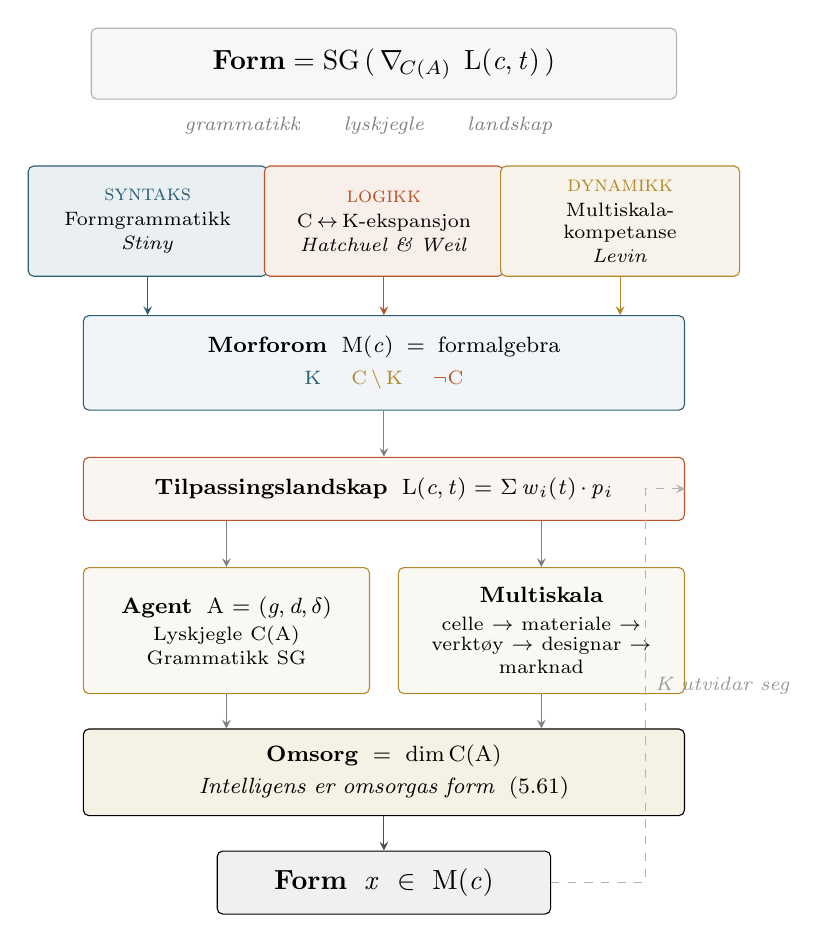
\begin{tikzpicture}[
  every node/.style={font=\footnotesize},
  box/.style={draw=#1, fill=#1!6, rounded corners=2pt,
              minimum height=8mm, text width=38mm, align=center,
              font=\footnotesize},
  pillar/.style={draw=#1, fill=#1!10, rounded corners=2pt,
                 minimum height=14mm, text width=28mm, align=center},
  arrow/.style={->, >=stealth, thin, #1},
  label/.style={font=\scriptsize\itshape, #1},
]

% ── Equation ──
\node[draw=black!30, fill=black!3, rounded corners=2pt,
      minimum height=9mm, text width=72mm, align=center]
  (eq) at (0, 8.2) {\normalsize\textbf{Form} = SG\,(\,$\nabla_{\!C(A)}$\, L(\textit{c},\,\textit{t})\,)};
\node[label=black!50, anchor=north] at (-1.8, 7.65) {grammatikk};
\node[label=black!50, anchor=north] at (0, 7.65) {lyskjegle};
\node[label=black!50, anchor=north] at (1.6, 7.65) {landskap};

% ── Three pillars ──
\definecolor{teal}{HTML}{2B5F75}
\definecolor{rust}{HTML}{B8542A}
\definecolor{gold}{HTML}{B4892A}

\node[pillar=teal] (sg) at (-3, 6.2)
  {\textsc{\color{teal}syntaks}\\[1pt]\scriptsize Formgrammatikk\\[-1pt]\scriptsize\textit{Stiny}};
\node[pillar=rust] (ck) at (0, 6.2)
  {\textsc{\color{rust}logikk}\\[1pt]\scriptsize C\,$\leftrightarrow$\,K-ekspansjon\\[-1pt]\scriptsize\textit{Hatchuel \& Weil}};
\node[pillar=gold] (tame) at (3, 6.2)
  {\textsc{\color{gold}dynamikk}\\[1pt]\scriptsize Multiskala-kompetanse\\[-1pt]\scriptsize\textit{Levin}};

% ── Morphospace ──
\node[box=teal, text width=74mm, minimum height=12mm] (morph) at (0, 4.4)
  {\textbf{Morforom}\; M(\textit{c})\;\;=\;\;formalgebra\\[2pt]
   \scriptsize\color{teal} K \quad\color{gold} C\,$\setminus$\,K \quad\color{rust} $\neg$C};

% ── Landscape ──
\node[box=rust, text width=74mm] (land) at (0, 2.8)
  {\textbf{Tilpassingslandskap}\; L(\textit{c},\,\textit{t}) = $\Sigma$\,\textit{w}$_i$(\textit{t})\,$\cdot$\,\textit{p}$_i$};

% ── Agent + Grammar ──
\node[box=gold, text width=34mm, minimum height=16mm] (agent) at (-2, 1.0)
  {\textbf{Agent}\; A = (\textit{g},\,\textit{d},\,\textit{$\delta$})\\[2pt]
   \scriptsize Lyskjegle C(A)\\[-1pt]
   \scriptsize Grammatikk SG};

% ── Multi-scale ──
\node[box=gold, text width=34mm, minimum height=16mm] (multi) at (2, 1.0)
  {\textbf{Multiskala}\\[2pt]
   \scriptsize celle $\to$ materiale $\to$\\[-1pt]
   \scriptsize verkt\o y $\to$ designar $\to$\\[-1pt]
   \scriptsize marknad};

% ── Care ──
\node[draw=black, fill=gold!12, rounded corners=2pt,
      minimum height=11mm, text width=74mm, align=center]
  (care) at (0, -0.8)
  {\textbf{Omsorg}\; =\; dim\,C(A)\\[2pt]
   \textit{Intelligens er omsorgas form}\;\;(5.61)};

% ── Form output ──
\node[draw=black, fill=black!6, rounded corners=2pt,
      minimum height=8mm, text width=40mm, align=center,
      font=\normalsize]
  (form) at (0, -2.2) {\textbf{Form}\; \textit{x}\; $\in$\; M(\textit{c})};

% ── Arrows ──
\draw[arrow=teal] (sg.south) -- (morph.north -| sg.south);
\draw[arrow=rust] (ck.south) -- (morph.north);
\draw[arrow=gold] (tame.south) -- (morph.north -| tame.south);

\draw[arrow=black!50] (morph.south) -- (land.north);
\draw[arrow=black!50] (land.south -| agent.north) -- (agent.north);
\draw[arrow=black!50] (land.south -| multi.north) -- (multi.north);

\draw[arrow=black!50] (agent.south) -- (care.north -| agent.south);
\draw[arrow=black!50] (multi.south) -- (care.north -| multi.south);
\draw[arrow=black!70] (care.south) -- (form.north);

% ── Feedback loop ──
\draw[arrow=black!30, dashed] (form.east) -- ++(1.2,0) |-
  node[pos=0.25, right, label=black!40] {K utvidar seg} (land.east);

\end{tikzpicture}
\end{figure}
 or compile standalone
\begin{figure}[p]
\centering
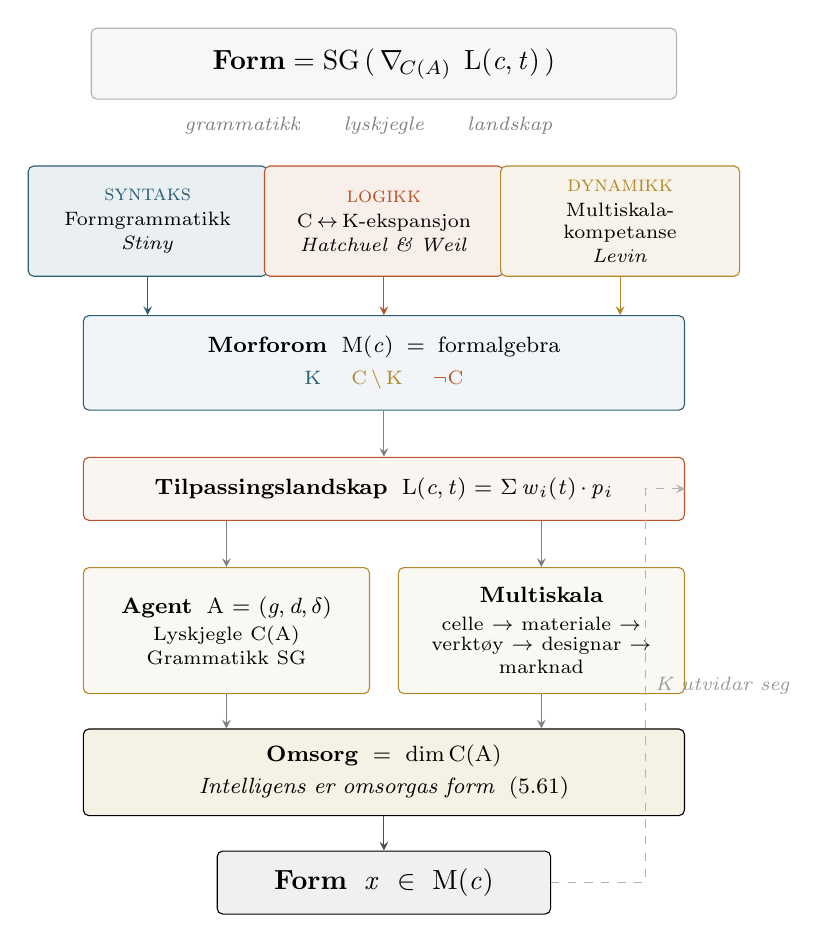
\begin{tikzpicture}[
  every node/.style={font=\footnotesize},
  box/.style={draw=#1, fill=#1!6, rounded corners=2pt,
              minimum height=8mm, text width=38mm, align=center,
              font=\footnotesize},
  pillar/.style={draw=#1, fill=#1!10, rounded corners=2pt,
                 minimum height=14mm, text width=28mm, align=center},
  arrow/.style={->, >=stealth, thin, #1},
  label/.style={font=\scriptsize\itshape, #1},
]

% ── Equation ──
\node[draw=black!30, fill=black!3, rounded corners=2pt,
      minimum height=9mm, text width=72mm, align=center]
  (eq) at (0, 8.2) {\normalsize\textbf{Form} = SG\,(\,$\nabla_{\!C(A)}$\, L(\textit{c},\,\textit{t})\,)};
\node[label=black!50, anchor=north] at (-1.8, 7.65) {grammatikk};
\node[label=black!50, anchor=north] at (0, 7.65) {lyskjegle};
\node[label=black!50, anchor=north] at (1.6, 7.65) {landskap};

% ── Three pillars ──
\definecolor{teal}{HTML}{2B5F75}
\definecolor{rust}{HTML}{B8542A}
\definecolor{gold}{HTML}{B4892A}

\node[pillar=teal] (sg) at (-3, 6.2)
  {\textsc{\color{teal}syntaks}\\[1pt]\scriptsize Formgrammatikk\\[-1pt]\scriptsize\textit{Stiny}};
\node[pillar=rust] (ck) at (0, 6.2)
  {\textsc{\color{rust}logikk}\\[1pt]\scriptsize C\,$\leftrightarrow$\,K-ekspansjon\\[-1pt]\scriptsize\textit{Hatchuel \& Weil}};
\node[pillar=gold] (tame) at (3, 6.2)
  {\textsc{\color{gold}dynamikk}\\[1pt]\scriptsize Multiskala-kompetanse\\[-1pt]\scriptsize\textit{Levin}};

% ── Morphospace ──
\node[box=teal, text width=74mm, minimum height=12mm] (morph) at (0, 4.4)
  {\textbf{Morforom}\; M(\textit{c})\;\;=\;\;formalgebra\\[2pt]
   \scriptsize\color{teal} K \quad\color{gold} C\,$\setminus$\,K \quad\color{rust} $\neg$C};

% ── Landscape ──
\node[box=rust, text width=74mm] (land) at (0, 2.8)
  {\textbf{Tilpassingslandskap}\; L(\textit{c},\,\textit{t}) = $\Sigma$\,\textit{w}$_i$(\textit{t})\,$\cdot$\,\textit{p}$_i$};

% ── Agent + Grammar ──
\node[box=gold, text width=34mm, minimum height=16mm] (agent) at (-2, 1.0)
  {\textbf{Agent}\; A = (\textit{g},\,\textit{d},\,\textit{$\delta$})\\[2pt]
   \scriptsize Lyskjegle C(A)\\[-1pt]
   \scriptsize Grammatikk SG};

% ── Multi-scale ──
\node[box=gold, text width=34mm, minimum height=16mm] (multi) at (2, 1.0)
  {\textbf{Multiskala}\\[2pt]
   \scriptsize celle $\to$ materiale $\to$\\[-1pt]
   \scriptsize verkt\o y $\to$ designar $\to$\\[-1pt]
   \scriptsize marknad};

% ── Care ──
\node[draw=black, fill=gold!12, rounded corners=2pt,
      minimum height=11mm, text width=74mm, align=center]
  (care) at (0, -0.8)
  {\textbf{Omsorg}\; =\; dim\,C(A)\\[2pt]
   \textit{Intelligens er omsorgas form}\;\;(5.61)};

% ── Form output ──
\node[draw=black, fill=black!6, rounded corners=2pt,
      minimum height=8mm, text width=40mm, align=center,
      font=\normalsize]
  (form) at (0, -2.2) {\textbf{Form}\; \textit{x}\; $\in$\; M(\textit{c})};

% ── Arrows ──
\draw[arrow=teal] (sg.south) -- (morph.north -| sg.south);
\draw[arrow=rust] (ck.south) -- (morph.north);
\draw[arrow=gold] (tame.south) -- (morph.north -| tame.south);

\draw[arrow=black!50] (morph.south) -- (land.north);
\draw[arrow=black!50] (land.south -| agent.north) -- (agent.north);
\draw[arrow=black!50] (land.south -| multi.north) -- (multi.north);

\draw[arrow=black!50] (agent.south) -- (care.north -| agent.south);
\draw[arrow=black!50] (multi.south) -- (care.north -| multi.south);
\draw[arrow=black!70] (care.south) -- (form.north);

% ── Feedback loop ──
\draw[arrow=black!30, dashed] (form.east) -- ++(1.2,0) |-
  node[pos=0.25, right, label=black!40] {K utvidar seg} (land.east);

\end{tikzpicture}
\end{figure}
 or compile standalone
\begin{figure}[p]
\centering
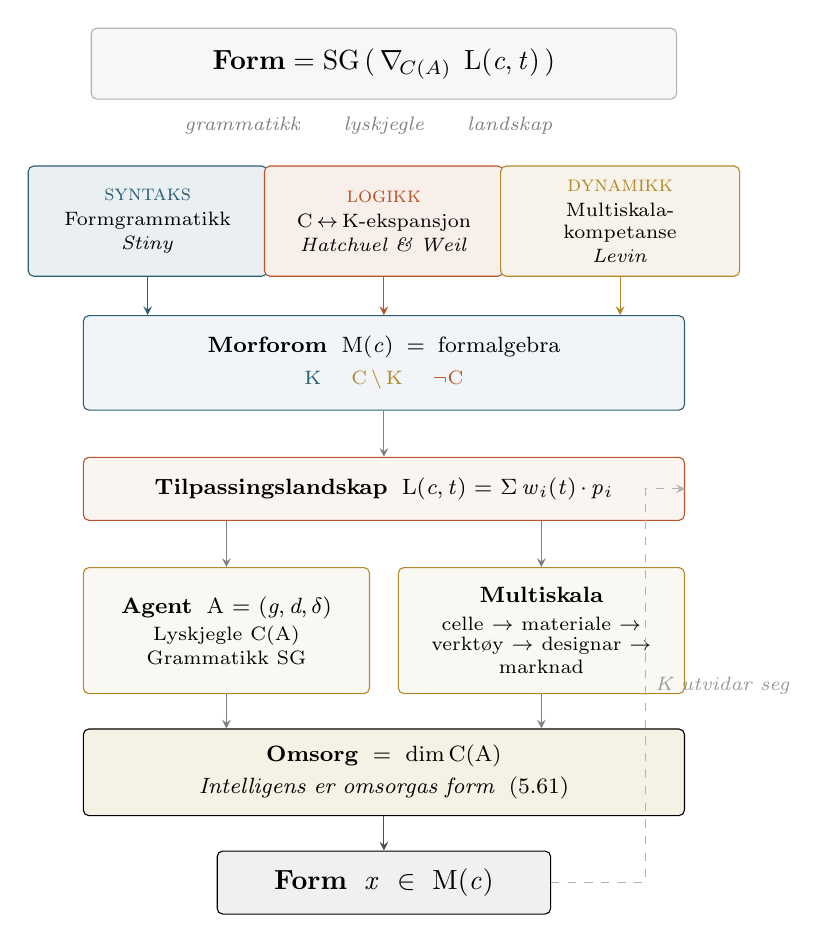
\begin{tikzpicture}[
  every node/.style={font=\footnotesize},
  box/.style={draw=#1, fill=#1!6, rounded corners=2pt,
              minimum height=8mm, text width=38mm, align=center,
              font=\footnotesize},
  pillar/.style={draw=#1, fill=#1!10, rounded corners=2pt,
                 minimum height=14mm, text width=28mm, align=center},
  arrow/.style={->, >=stealth, thin, #1},
  label/.style={font=\scriptsize\itshape, #1},
]

% ── Equation ──
\node[draw=black!30, fill=black!3, rounded corners=2pt,
      minimum height=9mm, text width=72mm, align=center]
  (eq) at (0, 8.2) {\normalsize\textbf{Form} = SG\,(\,$\nabla_{\!C(A)}$\, L(\textit{c},\,\textit{t})\,)};
\node[label=black!50, anchor=north] at (-1.8, 7.65) {grammatikk};
\node[label=black!50, anchor=north] at (0, 7.65) {lyskjegle};
\node[label=black!50, anchor=north] at (1.6, 7.65) {landskap};

% ── Three pillars ──
\definecolor{teal}{HTML}{2B5F75}
\definecolor{rust}{HTML}{B8542A}
\definecolor{gold}{HTML}{B4892A}

\node[pillar=teal] (sg) at (-3, 6.2)
  {\textsc{\color{teal}syntaks}\\[1pt]\scriptsize Formgrammatikk\\[-1pt]\scriptsize\textit{Stiny}};
\node[pillar=rust] (ck) at (0, 6.2)
  {\textsc{\color{rust}logikk}\\[1pt]\scriptsize C\,$\leftrightarrow$\,K-ekspansjon\\[-1pt]\scriptsize\textit{Hatchuel \& Weil}};
\node[pillar=gold] (tame) at (3, 6.2)
  {\textsc{\color{gold}dynamikk}\\[1pt]\scriptsize Multiskala-kompetanse\\[-1pt]\scriptsize\textit{Levin}};

% ── Morphospace ──
\node[box=teal, text width=74mm, minimum height=12mm] (morph) at (0, 4.4)
  {\textbf{Morforom}\; M(\textit{c})\;\;=\;\;formalgebra\\[2pt]
   \scriptsize\color{teal} K \quad\color{gold} C\,$\setminus$\,K \quad\color{rust} $\neg$C};

% ── Landscape ──
\node[box=rust, text width=74mm] (land) at (0, 2.8)
  {\textbf{Tilpassingslandskap}\; L(\textit{c},\,\textit{t}) = $\Sigma$\,\textit{w}$_i$(\textit{t})\,$\cdot$\,\textit{p}$_i$};

% ── Agent + Grammar ──
\node[box=gold, text width=34mm, minimum height=16mm] (agent) at (-2, 1.0)
  {\textbf{Agent}\; A = (\textit{g},\,\textit{d},\,\textit{$\delta$})\\[2pt]
   \scriptsize Lyskjegle C(A)\\[-1pt]
   \scriptsize Grammatikk SG};

% ── Multi-scale ──
\node[box=gold, text width=34mm, minimum height=16mm] (multi) at (2, 1.0)
  {\textbf{Multiskala}\\[2pt]
   \scriptsize celle $\to$ materiale $\to$\\[-1pt]
   \scriptsize verkt\o y $\to$ designar $\to$\\[-1pt]
   \scriptsize marknad};

% ── Care ──
\node[draw=black, fill=gold!12, rounded corners=2pt,
      minimum height=11mm, text width=74mm, align=center]
  (care) at (0, -0.8)
  {\textbf{Omsorg}\; =\; dim\,C(A)\\[2pt]
   \textit{Intelligens er omsorgas form}\;\;(5.61)};

% ── Form output ──
\node[draw=black, fill=black!6, rounded corners=2pt,
      minimum height=8mm, text width=40mm, align=center,
      font=\normalsize]
  (form) at (0, -2.2) {\textbf{Form}\; \textit{x}\; $\in$\; M(\textit{c})};

% ── Arrows ──
\draw[arrow=teal] (sg.south) -- (morph.north -| sg.south);
\draw[arrow=rust] (ck.south) -- (morph.north);
\draw[arrow=gold] (tame.south) -- (morph.north -| tame.south);

\draw[arrow=black!50] (morph.south) -- (land.north);
\draw[arrow=black!50] (land.south -| agent.north) -- (agent.north);
\draw[arrow=black!50] (land.south -| multi.north) -- (multi.north);

\draw[arrow=black!50] (agent.south) -- (care.north -| agent.south);
\draw[arrow=black!50] (multi.south) -- (care.north -| multi.south);
\draw[arrow=black!70] (care.south) -- (form.north);

% ── Feedback loop ──
\draw[arrow=black!30, dashed] (form.east) -- ++(1.2,0) |-
  node[pos=0.25, right, label=black!40] {K utvidar seg} (land.east);

\end{tikzpicture}
\end{figure}

